%% Template for MLP Coursework 1 / 14 October 2024 

%% Based on  LaTeX template for ICML 2017 - example_paper.tex at 
%%  https://2017.icml.cc/Conferences/2017/StyleAuthorInstructions

\documentclass{article}
\usepackage[T1]{fontenc}
\usepackage{amssymb,amsmath}
\usepackage{txfonts}
\usepackage{microtype}

% For figures
\usepackage{graphicx}
\usepackage{subcaption} 

% For citations
\usepackage{natbib}

% For algorithms
\usepackage{algorithm}
\usepackage{algorithmic}

% the hyperref package is used to produce hyperlinks in the
% resulting PDF.  If this breaks your system, please commend out the
% following usepackage line and replace \usepackage{mlp2017} with
% \usepackage[nohyperref]{mlp2017} below.
\usepackage{hyperref}
\usepackage{url}
\urlstyle{same}

\usepackage{color}
\usepackage{booktabs} % To thicken table lines
\usepackage{multirow} % Multirow cells in table
\usepackage{soul}
\usepackage{bm}

% Packages hyperref and algorithmic misbehave sometimes.  We can fix
% this with the following command.
\newcommand{\theHalgorithm}{\arabic{algorithm}}


% Set up MLP coursework style (based on ICML style)
\usepackage{mlp2022}
\mlptitlerunning{MLP Coursework 1 (\studentNumber)}
\bibliographystyle{icml2017}


\DeclareMathOperator{\softmax}{softmax}
\DeclareMathOperator{\sigmoid}{sigmoid}
\DeclareMathOperator{\sgn}{sgn}
\DeclareMathOperator{\relu}{relu}
\DeclareMathOperator{\lrelu}{lrelu}
\DeclareMathOperator{\elu}{elu}
\DeclareMathOperator{\selu}{selu}
\DeclareMathOperator{\maxout}{maxout}



\definecolor{red}{rgb}{0.95,0.4,0.4}
\definecolor{blue}{rgb}{0.4,0.4,0.95}
\definecolor{orange}{rgb}{1, 0.65, 0}

\newcommand{\youranswer}[1]{{\color{red} \bf[#1]}} %your answer: 


%% START of YOUR ANSWERS
%% REPLACE SXXXXXX with your student number
\def\studentNumber{SXXXXXX}


%% START of YOUR ANSWERS
%% Add answers to the questions below, by replacing the text inside the brackets {} for \youranswer{ "Text to be replaced with your answer." }. 
%
% Do not delete the commands for adding figures and tables. Instead fill in the missing values with your experiment results, and replace the images with your own respective figures.
%
% You can generally delete the placeholder text, such as for example the text "Question Figure 2 - Replace the images ..." 
%
% There are 18 TEXT QUESTIONS (a few of the short first ones have their answers added to both the Introduction and the Abstract). Replace the text inside the brackets of the command \youranswer with your answer to the question.
%
% There are also 3 "questions" to replace some placeholder FIGURES with your own, and 3 "questions" asking you to fill in the missing entries in the TABLES provided. 
%
% NOTE! that questions are ordered by the order of appearance of their answers in the text, and not by the order you should tackle them. Specifically, you cannot answer Questions 2, 3, and 4 before concluding all of the relevant experiments and analysis. Similarly, you should fill in the TABLES and FIGURES before discussing the results presented there. 
%
% NOTE! If for some reason you do not manage to produce results for some FIGURES and TABLES, then you can get partial marks by discussing your expectations of the results in the relevant TEXT QUESTIONS (for example Question 8 makes use of Table 1 and Figure 2).
%
% Please refer to the coursework specification for more details.


%% - - - - - - - - - - - - TEXT QUESTIONS - - - - - - - - - - - - 



%% Question 1:
\newcommand{\questionOne} {
\youranswer{Question 1 - Explain what these figures contain and how the curves evolve, and spot where overfitting occurs. Reason based on the min/max points and velocities (direction and magnitude of change) of the accuracy and error curves}
}

%% Question 2:
\newcommand{\questionTwo} {
\youranswer{Question 2 - Present your network width experiment results by using the relevant figure and table}
}

%% Question 3:
\newcommand{\questionThree} {
\youranswer{Question 3 - Discuss whether varying width affects the results in a consistent way, and whether the results are expected and match well with the prior knowledge (by which we mean your expectations as are formed from the relevant Theory and literature)}
}

%% Question 4:
\newcommand{\questionFour} {
\youranswer{Question 4 - Present your network depth experiment results by using the relevant figure and table}
}

%% Question 5:
\newcommand{\questionFive} {
\youranswer{Question 5 - Discuss whether varying depth affects the results in a consistent way, and whether the results are expected and match well with the prior knowledge (by which we mean your expectations as are formed from the relevant Theory and literature)}
}





%% Question 6:
\newcommand{\questionSix} {
\youranswer{Question 6 - Explain the experimental details (e.g. hyperparameters), discuss the results in terms of their generalisation performance and overfitting. Select and test the best performing model as part of this analysis.}
}

%% Question 7:
\newcommand{\questionSeven} {
\youranswer{Question 7 - Assume you were able to run 8 further training instances (8 specific hyperparameter configurations) where you could combine Dropout and L1, and/or Dropout and L2 regularisation. Which 8 runs would you pick and what question(s) would you aim to answer? Make sure you define the experiment setup, including any relevant hyperparameters}
}



%% Question 8:
\newcommand{\questionEight} {
\youranswer{Question 8 - Briefly draw your conclusions based on the results from the previous sections (what are the take-away messages?), discussing them in the context of the overall literature, and conclude your report with a recommendation for future directions}
}

%% - - - - - - - - - - - - FIGURES - - - - - - - - - - - - 

%% Question Figure 2:
\newcommand{\questionFigureTwo} {
\youranswer{Question Figure 2 - Replace the images in Figure 2 with figures depicting the accuracy and error, training and validation curves for your experiments varying the number of hidden units.
%
\begin{figure}[t]
    \centering
    \begin{subfigure}{\linewidth}
        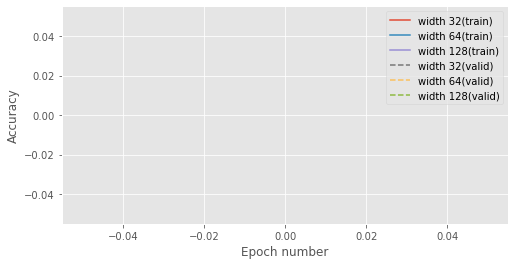
\includegraphics[width=\linewidth]{figures/empty_acc_curve_width.png}
        \caption{accuracy by epoch}
        \label{fig:width_acccurves}
    \end{subfigure} 
    \begin{subfigure}{\linewidth}
        \centering
        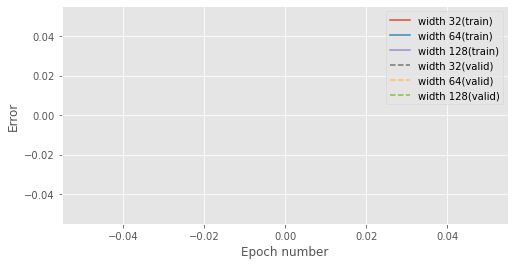
\includegraphics[width=\linewidth]{figures/empty_error_curve_width.png}
        \caption{error by epoch}
        \label{fig:width_errorcurves}
    \end{subfigure} 
    \caption{Training and validation curves in terms of classification accuracy (a) and cross-entropy error (b) on the EMNIST dataset for different network widths.}
    \label{fig:width}
\end{figure} 
}
}

%% Question Figure 3:
\newcommand{\questionFigureThree} {
\youranswer{Question Figure 3 - Replace these images with figures depicting the accuracy and error, training and validation curves for your experiments varying the number of hidden layers.
%
\begin{figure}[t]
    \centering
    \begin{subfigure}{\linewidth}
        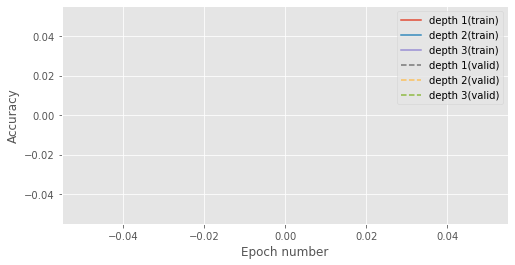
\includegraphics[width=\linewidth]{figures/empty_acc_curve_depth.png}
        \caption{accuracy by epoch}
        \label{fig:depth_acccurves}
    \end{subfigure} 
    \begin{subfigure}{\linewidth}
        \centering
        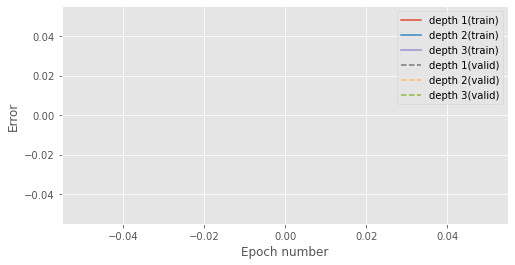
\includegraphics[width=\linewidth]{figures/empty_error_curve_depth.png}
        \caption{error by epoch}
        \label{fig:depth_errorcurves}
    \end{subfigure} 
    \caption{Training and validation curves in terms of classification accuracy (a) and cross-entropy error (b) on the EMNIST dataset for different network depths.}
    \label{fig:depth}
\end{figure} 
}
}

%% Question Figure 4:
\newcommand{\questionFigureFour} {
\youranswer{Question Figure 4 - Replace these images with figures depicting the Validation Accuracy and Generalisation Gap (difference between validation and training error) for each of the experiment results varying the Dropout inclusion rate, and L1/L2 weight penalty depicted in Table 3 (including any results you have filled in).
%
\begin{figure*}[t]
    \centering
    \begin{subfigure}{.475\linewidth}
        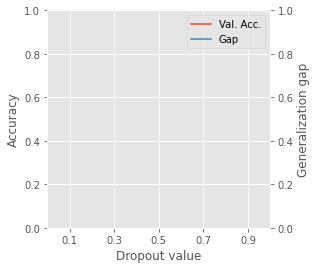
\includegraphics[width=\linewidth]{figures/empty_dropout_plot.png}
        \caption{Accuracy and error by inclusion probability.}
        \label{fig:dropoutrates}
    \end{subfigure} 
    \begin{subfigure}{.475\linewidth}
        \centering
        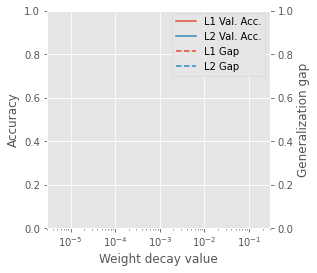
\includegraphics[width=\linewidth]{figures/empty_wd_plot.png}
        \caption{Accuracy and error by weight penalty.}
        \label{fig:weightrates}
    \end{subfigure} 
    \caption{Accuracy and error by regularisation strength of each method (Dropout and L1/L2 Regularisation).}
    \label{fig:hp_search}
\end{figure*}
}
}

%% - - - - - - - - - - - - TABLES - - - - - - - - - - - - 

%% Question Table 1:
\newcommand{\questionTableOne} {
\youranswer{
Question Table 1 - Fill in Table 1 with the results from your experiments varying the number of hidden units.
%
\begin{table}[t]
    \centering
    \begin{tabular}{c|ccc}
    \toprule
        \# Hidden Units & Val. Acc. & Train Error & Val. Error\\
    \midrule
         32            &    --.-   &  -.--- &   -.---            \\
         64            &    --.-   &  -.---  &   -.---               \\
         128           &    --.-   &  -.---  &   -.---           \\ 
    \bottomrule
    \end{tabular}
    \caption{Validation accuracy (\%) and training/validation error (in terms of cross-entropy error) for varying network widths on the EMNIST dataset.}
    \label{tab:width_exp}
\end{table}
}
}

%% Question Table 2:
\newcommand{\questionTableTwo} {
\youranswer{
Question Table 2 - Fill in Table 2 with the results from your experiments varying the number of hidden layers.
%
\begin{table}[t]
    \centering
    \begin{tabular}{c|ccc}
    \toprule
        \# Hidden Layers & Val. Acc. & Train Error & Val. Error \\
    \midrule
         1               &      --.-      &   -.--- & -.---                \\
         2               &      --.-      &   -.--- & -.---                \\
         3               &      --.-      &   -.--- & -.---                \\ 
    \bottomrule
    \end{tabular}
    \caption{Validation accuracy (\%) and training/validation error (in terms of cross-entropy error) for varying network depths on the EMNIST dataset.}
    \label{tab:depth_exps}
\end{table}
}
}

%% Question Table 3:
\newcommand{\questionTableThree} {
\youranswer{
Question Table 3 - Fill in Table 3 with the results from your experiments for the missing hyperparameter values for each of L1 regularisation, L2 regularisation, Dropout and label smoothing (use the values shown on the table).
%
\begin{table*}[t]
    \centering
    \begin{tabular}{c|c|ccc}
    \toprule
        Model    &  Hyperparameter value(s) & Validation accuracy & Train Error & Validation Error \\
    \midrule
    \midrule
        Baseline &  -                    &               0.837 &       0.241 &  0.533          \\
    \midrule
        \multirow{4}*{Dropout}
                 & 0.6                   &  80.7                &      0.549 & 0.593     \\
                 & 0.7 & --.- & -.--- & -.---  \\
                 & 0.85 & 85.1 &  0.329 &  0.434 \\
                 & 0.97 & 85.4 &  0.244 & 0.457  \\
    \midrule
        \multirow{4}*{L1 penalty}
                 & 5e-4 & 79.5 & 0.642 & 0.658 \\
                 & 1e-3 & --.- & -.--- & -.--- \\
                 & 5e-3 & 2.41 & 3.850 & 3.850 \\
                 & 5e-2 & 2.20 & 3.850 & 3.850 \\
    \midrule
        \multirow{4}*{L2 penalty}  
                 & 5e-4 & 85.1 & 0.306 & 0.460 \\
                 & 1e-3 & --.- & -.--- & -.--- \\
                 & 5e-3 & 81.3 & 0.586 & 0.607 \\
                 & 5e-2 & 39.2 & 2.258 & 2.256  \\
    \midrule
        Label smoothing & 0.1 & --.- & -.--- & -.--- \\
    \bottomrule
    \end{tabular}
    \caption{Results of all hyperparameter search experiments. \emph{italics} indicate the best results per series (Dropout, L1 Regularisation, L2 Regularisation, Label smoothing) and \textbf{bold} indicates the best overall.}
    \label{tab:hp_search}
\end{table*}
}
}

%% END of YOUR ANSWERS
%% END of YOUR ANSWERS



%% Do not change anything in this file. Add your answers to mlp-cw1-questions.tex



\begin{document} 

\twocolumn[
\mlptitle{MLP Coursework 1}
\centerline{\studentNumber}
\vskip 7mm
]


\begin{abstract} 
In this report we study the problem of overfitting, which is the training regime where performance increases on the training set but decrease on validation data. Overfitting prevents our trained model from generalizing well to unseen data.
We first analyse the given example and discuss the probable causes of the underlying problem. 
Then we investigate how the depth and width of a neural network can affect overfitting in a feedforward architecture and observe that increasing width and depth tend to enable further overfitting.
Next we discuss how two standard methods, Dropout and Weight Penalty, can
mitigate overfitting, then describe their implementation and use them in our experiments
to reduce the overfitting on the EMNIST dataset. 
Based on our results, we ultimately find that both dropout and weight penalty are able to mitigate overfitting.
Finally, we conclude the report with our observations and related work. 
Our main findings indicate that preventing overfitting is achievable through regularization, although combining different methods together is not straightforward.
\end{abstract} 


\section{Introduction}
\label{sec:intro}
In this report we focus on a common and important problem while training machine learning models known as overfitting, or overtraining, which is the training regime where performances increase on the training set but decrease on unseen data.
We first start with analysing the given problem in Figure~\ref{fig:example}, study it in different architectures and then investigate different strategies to mitigate the problem.
In particular, Section~\ref{sec:task1} identifies and discusses the given problem, and investigates the effect of network width and depth in terms of generalization gap (see Ch.~5 in \citealt{Goodfellow-et-al-2016}) and generalization performance.
Section \ref{sec:task2.1} introduces two regularization techniques to alleviate overfitting: Dropout \cite{srivastava2014dropout} and L1/L2 Weight Penalties (see Section~7.1 in \citealt{Goodfellow-et-al-2016}). 
We first explain them in detail and discuss why they are used for alleviating overfitting.
In Section~\ref{sec:task2.2}, we incorporate each of them and their various combinations to a three hidden layer\footnote{We denote all layers as hidden except the final (output) one. This means that depth of a network is equal to the number of its hidden layers + 1.} neural network, train it on the EMNIST dataset, which contains 131,600 images of characters and digits, each of size 28x28, from 47 classes.
We evaluate them in terms of generalization gap and performance, and discuss the results and effectiveness of the tested regularization strategies.
Our results show that both dropout and weight penalty are able to mitigate overfitting.

Finally, we conclude our study in Section~\ref{sec:concl}, noting that preventing overfitting is achievable through regularization, although combining different methods together is not straightforward.


\section{Problem identification}
\label{sec:task1}

\begin{figure}[t]
    \centering
    \begin{subfigure}{\linewidth}
        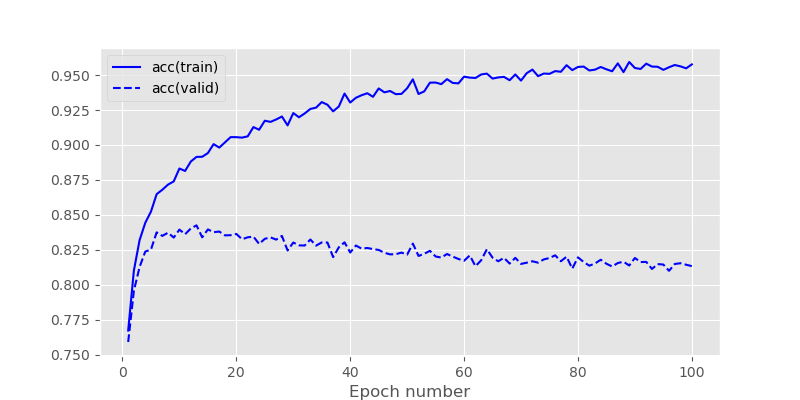
\includegraphics[width=\linewidth]{figures/fig1_acc.png}
        \caption{accuracy by epoch}
        \label{fig:example_acccurves}
    \end{subfigure} 
    \begin{subfigure}{\linewidth}
        \centering
        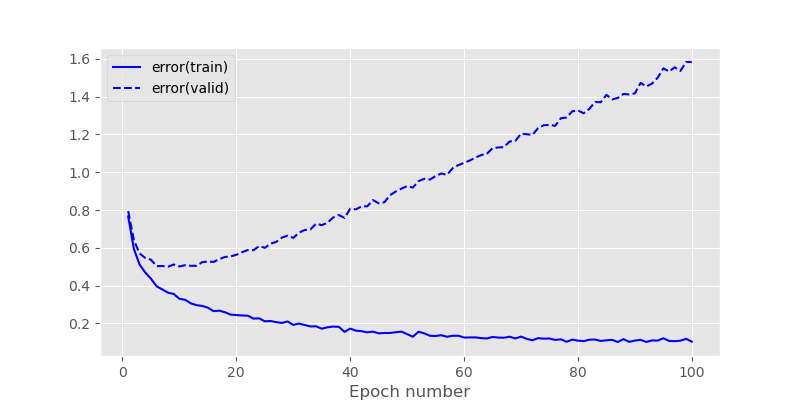
\includegraphics[width=\linewidth]{figures/fig1_err.png}
        \caption{error by epoch}
        \label{fig:example_errorcurves}
    \end{subfigure} 
    \caption{Training and validation curves in terms of classification accuracy (a) and cross-entropy error (b) on the EMNIST dataset for the baseline model.}
    \label{fig:example}
\end{figure} 

Overfitting to training data is a very common and important issue that needs to be dealt with when training neural networks or other machine learning models in general (see Ch.~5 in \citealt{Goodfellow-et-al-2016}).
A model is said to be overfitting when as the training progresses, its performance on the training data keeps improving, while its is degrading on validation data. 
Effectively, the model stops learning related patterns for the task and instead starts to memorize specificities of each training sample that are irrelevant to new samples. 
Overfitting leads to bad generalization performance in unseen data, as performance on validation data is indicative of performance on test data and (to an extent) during deployment.

Although it eventually happens to all gradient-based training, it is most often caused by models that are too large with respect to the amount and diversity of training data. The more free parameters the model has, the easier it will be to memorize complex data patterns that only apply to a restricted amount of samples.
A prominent symptom of overfitting is the generalization gap, defined as the difference between the validation and training error. 
A steady increase in this quantity is usually interpreted as the model entering the overfitting regime.


Figure~\ref{fig:example_acccurves} and \ref{fig:example_errorcurves} show a prototypical example of overfitting.
We see in Figure~\ref{fig:example_acccurves} that \questionOne.

The extent to which our model overfits depends on many factors.
For example, the quality and quantity of the training set and the complexity of the model. 
If we have sufficiently many diverse training samples, or if our model contains few hidden units, it will in general be less prone to overfitting. 
Any form of regularization will also limit the extent to which the model overfits.


\subsection{Network width}

\questionTableOne
\questionFigureTwo

First we investigate the effect of increasing the number of hidden units in a single hidden layer network when training on the EMNIST dataset.
The network is trained using the Adam optimizer
with a learning rate of $9 \times 10^{-4}$ and a batch size of 100, for a total of 100 epochs.

The input layer is of size 784, and output layer consists of 47 units. 
Three different models were trained, with a single hidden layer of 32, 64 and 128 ReLU hidden units respectively.
Figure~\ref{fig:width} depicts the error and accuracy curves over 100 epochs for the model with varying number of hidden units.
Table~\ref{tab:width_exp} reports the final accuracy, training error, and validation error.
We observe that \questionTwo.

\questionThree.


\subsection{Network depth}

\questionTableTwo
\questionFigureThree

Next we investigate the effect of varying the number of hidden layers in the network. 
Table~\ref{tab:depth_exps} and Figure~\ref{fig:depth} depict results from training three models with one, two and three hidden layers respectively, each with 128 ReLU hidden units. 
As with previous experiments, they are trained with the Adam optimizer with a learning rate of $9 \times 10^{-4}$ and a batch size of 100. 

We observe that \questionFour.

\questionFive.




\section{Regularization}
\label{sec:task2.1} 

In this section, we investigate three regularization methods to alleviate the overfitting problem, specifically dropout layers, the L1 and L2 weight penalties and label smoothing.


\subsection{Dropout}

Dropout~\cite{srivastava2014dropout} is a stochastic method that randomly inactivates neurons in a neural network according to an hyperparameter, the inclusion rate  (\textit{i.e.} the rate that an unit is included).
Dropout is commonly represented by an additional layer inserted between the linear layer and activation function.
Its forward pass during training is defined as follows:
\begin{align}
    \text{mask} &\sim \text{bernoulli}(p)\\
    \bm{y}' &= \text{mask} \odot \bm{y}\
\end{align}
where $\bm{y}, \bm{y}' \in \mathbb{R}^d$ are the output of the linear layer before and after applying dropout, respectively. 
$\text{mask} \in \mathbb{R}^d$ is a mask vector randomly sampled from the Bernoulli distribution with inclusion probability $p$, and $\odot$ denotes the element-wise multiplication.

At inference time, stochasticity is not desired, so no neurons are dropped. 
To account for the change in expectations of the output values, we scale them down by the inclusion probability $p$:
\begin{align}
    \bm{y}' &= \bm{y}*p\
\end{align}

As there is no nonlinear calculation involved, the backward propagation is just the element-wise product of the gradients with respect to the layer outputs and mask created in the forward calculation. 
The backward propagation for dropout is therefore formulated as follows:
\begin{align}
    \frac{\partial \bm{y}'}{\partial \bm{y}} = mask
\end{align}

Dropout is an easy to implement and highly scalable method. 
It can be implemented as a layer-based calculation unit, and be placed on any layer of the neural network at will. 
Dropout can reduce the dependence of hidden units between layers so that the neurons of the next layer will not rely on only few features from of the previous layer.
Instead, it forces the network to extract diverse features and evenly distribute information among all features. 
By randomly dropping some neurons in training, dropout makes use of a subset of the whole architecture, so it can also be viewed as bagging different sub networks and averaging their outputs.


\subsection{Weight penalty}

L1 and L2 regularization~\cite{ng2004feature} are simple but effective methods to mitigate overfitting to training data. 
The application of L1 and L2 regularization strategies could be formulated as adding penalty terms with L1 and L2 norm square of weights in the cost function without changing other formulations. 
The idea behind this regularization method is to penalize the weights by adding a term to the cost function, and explicitly constrain the magnitude of the weights with either the L1 and L2 norms.
The optimization problem takes a different form:
\begin{align}
    \text{L1: } & \text{min}_{\bm{w}} \; E_{\text{data}}(\bm{X}, \bm{y}, \bm{w}) + \lambda ||w||_1\\
    \text{L2: } & \text{min}_{\bm{w}} \; E_{\text{data}}(\bm{X}, \bm{y}, \bm{w}) + \lambda ||w||^2_2
\end{align}
where $E_{\text{data}}$ denotes the cross entropy error function, and $\{\bm{X}, \bm{y}\}$ denotes the input and target training pairs. 
$\lambda$ controls the strength of regularization.

Weight penalty works by constraining the scale of parameters and preventing them to grow too much, avoiding overly sensitive behaviour on unseen data.
While L1 and L2 regularization are similar to each other in calculation, they have different effects.
Gradient magnitude in L1 regularization does not depend on the weight value and tends to bring small weights to 0, which can be used as a form of feature selection, whereas L2 regularization tends to shrink the weights to a smaller scale uniformly. 


\subsection{Label smoothing}
Label smoothing regularizes a model based on a softmax with $K$ output values by replacing the hard target 0 labels and 1 labels with $\frac{\alpha}{K-1}$ and $1-\alpha$ respectively. 
$\alpha$ is typically set to a small number such as $0.1$.
\begin{equation}
    \begin{cases}
        \frac{\alpha}{K-1}, & \quad \text{if} \quad t_k=0\\
        1 - \alpha, & \quad \text{if} \quad t_k=1
    \end{cases}    
\end{equation}
The standard cross-entropy error is typically used with these \emph{soft} targets to train the neural network. 
Hence, implementing label smoothing requires only modifying the targets of training set.
This strategy may prevent a neural network to obtain very large weights by discouraging very high output values.

\section{Balanced EMNIST Experiments}

\questionTableThree

\questionFigureFour

\label{sec:task2.2}

Here we evaluate the effectiveness of the given regularization methods for reducing the overfitting on the EMNIST dataset.
We build a baseline architecture with three hidden layers, each with 128 neurons, which suffers from overfitting as shown in section \ref{sec:task1}.

Here we train the network with a lower learning rate of $10^{-4}$, as the previous runs were overfitting after only a handful of epochs. 
Results for the new baseline (c.f. Table~\ref{tab:hp_search}) confirm that lower learning rate helps, so all further experiments are run using it.

Here, we apply the L1 or L2 regularization with dropout to our baseline and search for good hyperparameters on the validation set. 
Then, we apply the label smoothing with $\alpha=0.1$ to our baseline.
We summarize all the experimental results in Table~\ref{tab:hp_search}. For each method except the label smoothing, we plot the relationship between generalization gap and validation accuracy in Figure~\ref{fig:hp_search}.

First we analyze three methods separately, train each over a set of hyperparameters and compare their best performing results.

\questionSix.

\questionSeven.


\section{Conclusion}
\label{sec:concl}
    
\questionEight.

\newpage
\bibliography{refs}

\end{document} 

